%   % !TEX root = ../../VIII,3_Rahmen-TeX_9-0.tex
%  
%   Signatur/Tex-Datei:	LH_35_09_22_001-002
%   RK-Nr. 	41206
%   Überschrift: 	De concursu sine ictu, deque refractione etc.
%   Datierung:		19. November 1681 (a. St.), eigh.
%   WZ: 	Bl. 1, Nr. 803045 								
%   edlabels:	 		4
%   Diagramme: 		9
%
%
\selectlanguage{ngerman}
\frenchspacing
%
\begin{ledgroupsized}[r]{120mm}
\footnotesize
\pstart
\noindent\textbf{Überlieferung:}
\pend
\end{ledgroupsized}
%
\begin{ledgroupsized}[r]{114mm}
\footnotesize
\pstart \parindent -6mm
\makebox[6mm][l]{\textit{L}}%
Konzept:
LH~XXXV~9, 22 Bl.~1\textendash2.
Ein Bogen~2\textsuperscript{o};
Wasserzeichen auf Bl.~1.
Zwei Seiten auf Bl.~1; Bl.~2 leer.
Leibniz hat die Passage auf S.~\refpassage{35_09_22_001-002_4a}{35_09_22_001-002_4b} in einem weiteren, ebenfalls auf den 19.\ (29.) November datierten Stück, \glqq De refractione pilae\grqq\ (LH~XXXV~9, 22 Bl.~4\textendash5) überarbeitet. Das Stück erscheint in einem späteren Band der Reihe.
\pend
\end{ledgroupsized}
%
\selectlanguage{latin}
\frenchspacing
%
\vspace{8mm}
\pstart%
\normalsize%
\noindent%
\lbrack 1~r\textsuperscript{o}\rbrack\
\pend
%
\pstart
\noindent%
\raggedleft
%
\edlabel{35_09_22_001-002_1a}%
\edtext{}{% NEUER ABSATZ UND ERGÄNZUNG
{\xxref%
{35_09_22_001-002_1a}{35_09_22_001-002_1b}}%
\lemma{}%
\Bfootnote{%
19. Novemb. \lbrack...\rbrack\ etc. \textit{erg.}~\textit{L}}}%
19. Novemb. 1681.
\pend
%
\pstart
\centering%
De concursu sine ictu,%
\protect\index{Sachverzeichnis}{concursus sine ictu}
%
deque refractione.\protect\index{Sachverzeichnis}{refractio} etc.%
\edlabel{35_09_22_001-002_1b}
\pend%
\vspace{0.5em}
%
\vspace{1.5em} %Diagramme 1 und 2 (ehem 1.1, 1.2). Bitte an K.Zeitz: Diagramme 1 und 2 sollen nebeneinander bleiben.
\centerline{%
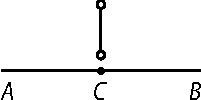
\includegraphics[width=0.25\textwidth]{%
gesamttex/edit_VIII,3/images/LH_35_09_22_001-002_d1_001r.pdf%
}%
\hspace*{25mm}%
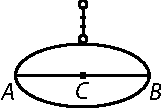
\includegraphics[width=0.19\textwidth]{%
gesamttex/edit_VIII,3/images/LH_35_09_22_001-002_d2_001r.pdf}%
}
\vspace{0.5em}
\centerline{%
\hspace*{5mm}\lbrack\textit{Fig.~1}\rbrack \hspace*{40mm} \lbrack\textit{Fig.~2}\rbrack\hspace*{0mm}%
}
\vspace{1.5em}
%
\pstart
\noindent
\edtext{Si corpori \textit{AB} homogeneo\protect\index{Sachverzeichnis}{corpus homogeneum}}{\lemma{Si}%
\Bfootnote{%
\textit{(1)}~rectae \textit{AB} homogeneae %
\textit{(2)}~corpori \textit{AB} homogeneo~\textit{L}}}
%
\edtext{centrum magnitudinis\protect\index{Sachverzeichnis}{centrum magnitudinis} habenti}{\lemma{centrum}%
\Bfootnote{magnitudinis habenti %
\textit{erg.}~\textit{L}}}
%
impetus\protect\index{Sachverzeichnis}{impetus} imprimatur directus in
%
\edtext{centrum \textit{C},}{\lemma{}%
\Bfootnote{centrum \textbar\ gravitatis \textit{gestr.}~\textbar\ \textit{C},~\textit{L}}}
%
omnia ejus puncta ferentur linea lineae motus centri gravitatis\protect\index{Sachverzeichnis}{motus centri gravitatis}
%
\edlabel{35_09_22_001-002_2a}%
\edtext{}{% NEUER ABSATZ UND VARIANTEN – "parallela... Impetus autem"
{\xxref%
{35_09_22_001-002_2a}{35_09_22_001-002_2b}}%
\lemma{parallela.}%
\Bfootnote{%
\textit{(1)}~Lineam autem parallelam intelligo, cum tangentes respondentes sunt parallelae. Impetus impressus intelli %
\textit{(2)}~Hoc manifestum \lbrack...\rbrack\ Impetus autem~\textit{L}}}%
parallela. Hoc manifestum est, quia nulla est ratio diversitatis.
\pend
%
\vspace{1.5em} %Diagramm 3, ehem 2
\centerline{%
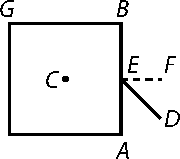
\includegraphics[width=0.2\textwidth]{%
gesamttex/edit_VIII,3/images/LH_35_09_22_001-002_d3_001r.pdf%
}} 
\vspace{0.5em}
\centerline{%
\lbrack\textit{Fig.~3}\rbrack%
}
\vspace{1.5em}
%
\pstart
Impetus autem\edlabel{35_09_22_001-002_2b}
%
impressus%
\protect\index{Sachverzeichnis}{impetus impressus}
%
intelligitur secundum perpendicularem ad superficiem. Ut
%
\edtext{si impetus\protect\index{Sachverzeichnis}{impetus}}{\lemma{si}%
\Bfootnote{\textit{(1)}~mobile d \textit{(2)}~impetus~\textit{L}}}
%
directione \textit{DE} imprimatur quadrato \textit{AG}, in puncto \textit{E}, medio lateris 
%
\edtext{\lbrack\textit{BA}\rbrack,}{%
\lemma{}%
\Bfootnote{%
\textit{DE} %
\textit{L ändert Hrsg.}%
}}
%
tunc
%
\edtext{licet recta}{\lemma{licet}\Bfootnote{\textit{(1)}~angulus \textit{(2)}~recta~\textit{L}}}
%
\textit{DE} continuata non perveniat in centrum quadrati, tamen, quia angulus est obliquus,
%
\edtext{et impressio\protect\index{Sachverzeichnis}{impressio}}{\lemma{et}%
\Bfootnote{\textit{(1)}~vis \textit{(2)}~impressio~\textit{L}}}
%
in perpendiculari \textit{FE} facta
%
\edtext{intelligitur quae}{%
\lemma{intelligitur}%
\Bfootnote{%
\textit{(1)}~ideo %
\textit{(2)}~quae~\textit{L}}}
%
continuata ad centrum pervenit; ideo impressio\protect\index{Sachverzeichnis}{impressio} in
%
centrum gravitatis\protect\index{Sachverzeichnis}{centrum gravitatis} directa
%
\edlabel{35_09_22_001-002_3a}%
\edtext{}{% NEUER ABSATZ UND VARIANTEN – "Videtur. Igitur"
{\xxref%
{35_09_22_001-002_3a}{35_09_22_001-002_3b}}%
\lemma{videtur.}%
\Bfootnote{%
\textit{(1)}~Ideo %
\textit{(2)}~Igitur~\textit{L}}}%
videtur.
\pend
%
\pstart
Igitur
\edlabel{35_09_22_001-002_3b}
%
si impetus\protect\index{Sachverzeichnis}{impetus}
%
\edtext{corpori impressus\protect\index{Sachverzeichnis}{impetus impressus}}{\lemma{}%
\Bfootnote{corpori \textbar\ aliquo \textit{gestr.}~\textbar\ impressus~\textit{L}}}
%
intelligatur \edtext{in puncto}{\lemma{}\Bfootnote{in puncto \textit{erg.}~\textit{L}}}
%
ubi perpendicularis ad planum tangens producta in centrum gravitatis\protect\index{Sachverzeichnis}{centrum gravitatis}
%
pervenit, impetus\protect\index{Sachverzeichnis}{impetus} in centrum gravitatis\protect\index{Sachverzeichnis}{centrum gravitatis} 
%
\edtext{directus erit,}{\lemma{directus}%
\Bfootnote{\textit{(1)}~videbitur \textit{(2)}~erit,~\textit{L}}}
%
et contra.\pend 
%
\vspace{1.0em} %Diagramm 4 ehem 3 
\centerline{%
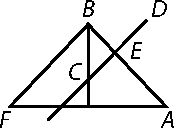
\includegraphics[width=0.21\textwidth]{%
gesamttex/edit_VIII,3/images/LH_35_09_22_001-002_d4_001r.pdf%
}} 
\vspace{0.5em}
\centerline{%
\lbrack\textit{Fig.~4}\rbrack%
}
\vspace{1em}
%
\pstart
Si corpus homogeneum%
\protect\index{Sachverzeichnis}{corpus homogeneum}
%
 quidem sit nullum tamen habeat centrum magnitudinis,%
\protect\index{Sachverzeichnis}{centrum magnitudinis}
%
 ut triangulum rectangulum, idem tamen
%
\edtext{dicendum esse videtur,}{\lemma{dicendum}%
\Bfootnote{\textit{(1)}~erit, \textit{(2)}~esse videtur,~\textit{L}}}
%
si animum abstrahamus a resistentia medii\protect\index{Sachverzeichnis}{resistentia medii}. Impetus\protect\index{Sachverzeichnis}{impetus} 
%
enim idem aeque omnibus punctis imprimi videtur.
\pend
%
\pstart
Secus tamen est, si tale corpus feratur in medio resistente\lbrack:\rbrack%
\protect\index{Sachverzeichnis}{medium resistens}
%
tunc enim idem est, an in ipsum quiescens
%
ventus%
\protect\index{Sachverzeichnis}{ventus}
%
 flet motui ejus prius posito contrarius. Is enim potest ita in corpus incidere ut ipsum circumagat. 
\pend 
%
\vspace{1.0em} %Diagramm 5 ehem 4.1
\centerline{%
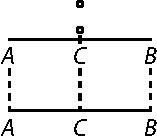
\includegraphics[width=0.20\textwidth]{%
gesamttex/edit_VIII,3/images/LH_35_09_22_001-002_d5_001r.pdf%
}} 
\vspace{0.5em}
\centerline{%
\lbrack\textit{Fig.~5}\rbrack%
}
% \newpage%
\vspace{1em}
%
\pstart
Sed satius erit nondum progredi
%
\edtext{ad composita\protect\index{Sachverzeichnis}{compositum}}{\lemma{}%
\Bfootnote{ad \textbar\ corpora \textit{gestr.} \textbar\ composita~\textit{L}}}
%
nimis et prius lineam
%
\edtext{rectam homogeneam\protect\index{Sachverzeichnis}{linea recta homogenea}}{\lemma{}\Bfootnote{homogeneam \textit{erg.}~\textit{L}}}
%
satis examinare. Cui si \edtext{impetus\protect\index{Sachverzeichnis}{impetus} imprimatur}{\lemma{impetus}%
\Bfootnote{\textit{(1)}~per \textit{(2)}~imprimatur~\textit{L}}}
%
in puncto medio, utique omnia puncta medio parallela ferentur.
\pend 
% 
\vspace{1.0em} %Diagramm 6 ehem 4.2
\centerline{%
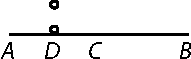
\includegraphics[width=0.21\textwidth]{%
gesamttex/edit_VIII,3/images/LH_35_09_22_001-002_d6_001r.pdf%
}} 
\vspace{0.5em}
\centerline{%
\lbrack\textit{Fig.~6}\rbrack%
}
\vspace{1em}
%
\pstart 
Sed quid si impetus\protect\index{Sachverzeichnis}{impetus} imprimatur alteri cuidam puncto 
%
\edtext{\textit{D}.}{%
\lemma{}%
\Bfootnote{%
\textit{D} %
\textit{erg.~L}}}
%
Paulo aliter ratiocinandum, et considerandum quo corpus sit majus, hoc ferri tardius.
%
Itaque si ponamus \textit{D} medium inter \textit{A} et \textit{C},
%
\edtext{hinc \textit{AC}}{\lemma{hinc}%
\Bfootnote{\textit{(1)}~tota \textit{(2)}~\textit{AC}~\textit{L}}}
%
celerius utique ferretur; si a \textit{CB} esset separata, ea autem \textit{AC} haud dubie ferretur omnibus punctis 
%
\edtext{ipsi \textit{D}}{\lemma{ipsi}%
\Bfootnote{\textit{(1)}~\textit{C} \textit{(2)}~\textit{D}~\textit{L}}}
%
parallelis. Nunc autem cum \textit{CB} secum abripere debeat, quod motum retardat, ideo \textit{AC},
%
celerius progredietur, \textit{CB} tardius, et remotior ipsius \textit{CB} pars tardissime.
%
Ita enim impetus ipsius \textit{CB}, quam celerrime
%
\edtext{procedendi,\protect\index{Sachverzeichnis}{impetus quam celerrime procedendi} quemadmodum}{\lemma{procedendi,}%
\Bfootnote{\textit{(1)}~esse \textit{(2)}~quemadmodum~\textit{L}}}
%
fert impetus impressus\protect\index{Sachverzeichnis}{impetus impressus}, effectum suum consequetur, ideo simul et 
%
progredietur linea \textit{AB}, et movebitur circa centrum \textit{B}. Nam punctum \textit{B} et alia, cum etiam 
%
impetum\protect\index{Sachverzeichnis}{impetus} recipiant, nonnhihil progredi debent, licet tardius.
\pend 
%
\pstart
Quaeritur determinatio huius motus.
\pend
%
%
\vspace{1.5em} %Diagramm 7 ehem 5
\centerline{%
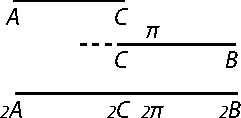
\includegraphics[width=0.28\textwidth]{%
gesamttex/edit_VIII,3/images/LH_35_09_22_001-002_d7_001r.pdf%
}} 
\vspace{0.5em}
\centerline{%
\lbrack\textit{Fig.~7}\rbrack%
}
% \newpage%
\vspace{1em}
%
\pstart
Considerandum autem fore circularem
%
\edtext{motum\protect\index{Sachverzeichnis}{motus circularis} eo}{\lemma{motum}%
\Bfootnote{\textit{(1)}~tanto \textit{(2)}~eo~\textit{L}}}
%
minorem et parallelum%
\protect\index{Sachverzeichnis}{motus parallelus}
%
 eo majorem quo propius est punctum \textit{D} puncto \textit{C}. Solutio huius quaestionis ita haberi posse videtur.
%
Ponamus \textit{AC} procedere, et incidens in \textit{CB} linea indivisibili%
\protect\index{Sachverzeichnis}{linea indivisibilis}
%
ipsum apprehendere
%
\edtext{vel glutine\protect\index{Sachverzeichnis}{gluten}}{\lemma{}%
\Bfootnote{vel glutine \textit{erg.}~\textit{L}}}
%
secumque rapere, et in unum coire\lbrack:\rbrack\ primum, centrum gravitatis
%
\edtext{$\pi$}{%
\lemma{$\pi$}%
\Bfootnote{%
\textit{} %
\textit{erg.~L}}}
%
commune%
\protect\index{Sachverzeichnis}{centrum gravitatis commune}
%
post concursum eo modo procedet quo ante concursum.
%
\edtext{Deinde totum}{\lemma{Deinde}%
\Bfootnote{\textit{(1)}~ambo m \textit{(2)}~totum~\textit{L}}} 
%
moveatur \edtext{eo modo in \textit{AB},}{%
\lemma{eo modo}%
\Bfootnote{%
\textit{(1)}~\textbar\ ex \textit{streicht Hrsg.}~\textbar\ \textit{A} %
\textit{(2)}~in \textit{AB},~\textit{L}}}
%
ut si post progressionem totius aliquam
%
rupto glutine\protect\index{Sachverzeichnis}{gluten} a se invicem liberentur, et unum quodque coepto 
%
impetu\protect\index{Sachverzeichnis}{impetus} pergat, aggregatum potentiarum%
\protect\index{Sachverzeichnis}{aggregatum potentiae} 
%
\lbrack1~v\textsuperscript{o}\rbrack\ aequetur potentiae totius.%
\protect\index{Sachverzeichnis}{potentia totius}
\pend
%
\pstart
Et hinc puto determinari posse quaesitum.
\pend
%
\vspace{1.5em} %Diagramm 8 ehem 6
\centerline{%

\includegraphics[width=0.25\textwidth]{%
gesamttex/edit_VIII,3/images/LH_35_09_22_001-002_d8_001v.pdf%
}} 
\vspace{0.5em}
\centerline{%
\lbrack\textit{Fig.~8}\rbrack%
}
\vspace{1em}
%
\pstart
%
\hspace{1mm}\hspace{-1mm}% Trick, weil \edlabel nicht zu \par-Beginn sein darf
\edlabel{35_09_22_001-002_4a}%
Eodem modo et si ventus%
\protect\index{Sachverzeichnis}{ventus}
%
 impellat corpus \textit{AML} cujus pars \textit{AM} sit lignea, \textit{ML} ferrea\lbrack:\rbrack\ etiam inclinabitur
%
in partem \edtext{\lbrack ligneam\rbrack,}{%
\lemma{}%
\Bfootnote{%
ligneae %
\textit{L ändert Hrsg.}}}
%
quod eodem modo efficietur fingendo ambo ferri suo impetu\protect\index{Sachverzeichnis}{impetus}, quem si solum esset a vento,%
\protect\index{Sachverzeichnis}{ventus}
%
accepisset et denique in unum coalescere se praetereundo. Manebit via centri gravitatis%
\protect\index{Sachverzeichnis}{via centri gravitatis}
%
eadem quae ante; et
%
\edtext{praeterea angulus\protect\index{Sachverzeichnis}{angulus}}{\lemma{praeterea}%
\Bfootnote{\textit{(1)}~potentia quoque singulorum \textit{(2)}~angulus~\textit{L}}}
%
quoque, \edtext{si assumatur}{\lemma{si}%
\Bfootnote{\textit{(1)}~qualis \textit{(2)}~assumatur~\textit{L}}}
%
aliquis, et post aliquem progressum indefinite parvum%
\protect\index{Sachverzeichnis}{progressus indefinite parvus}
%
rursus a se invicem liberentur\lbrack,\rbrack\
%
et aggregatum potentiae%
\protect\index{Sachverzeichnis}{aggregatum potentiae}
%
\edtext{\lbrack erit\rbrack}{%
\lemma{}%
\Bfootnote{%
sit %
\textit{L ändert Hrsg.}}}
% 
idem quod ante.
%
Vereor tamen, ut ex hoc aggregato potentiae%
\protect\index{Sachverzeichnis}{aggregatum potentiae}
%
oriatur aliquid novi,
%
quamquam nova hoc modo oriri videam, in investigatione eorum quae post conflictus\protect\index{Sachverzeichnis}{conflictus} contingunt.
\pend 
%
\vspace{1.5em} %Diagramm 9 ehem 7 %%%%%%%%%%%%
\centerline{%
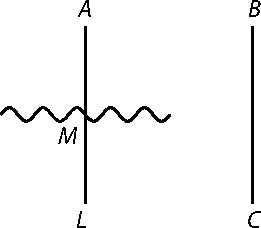
\includegraphics[width=0.31\textwidth]{%
gesamttex/edit_VIII,3/images/LH_35_09_22_001-002_d9_001v.pdf%
}} 
\vspace{0.5em}
\centerline{%
\lbrack\textit{Fig.~9}\rbrack%
}
% \newpage%
\vspace{1em}
%
\pstart
Quodsi ponamus \edtext{stipitem\protect\index{Sachverzeichnis}{stipes} erectum}{\lemma{stipitem}\Bfootnote{%
\textit{(1)}~partim %%
\textit{(a)}~int %
\textit{(b)}~in a %
\textit{(2)}~erectum~\textit{L}}}
partim in aqua esse mersum, partim in aere extare, et ita moveri ab aliquo verbi gratia
%
si ferreus aut ferro sit circumdatus, a magnete\protect\index{Sachverzeichnis}{magnes}
%
\edtext{\textit{BC}}{%
\lemma{}%
\Bfootnote{%
\textit{BC} %
\textit{erg.~L}}}
%
attrahi \edtext{ubi pars}{\lemma{ubi}%
\Bfootnote{\textit{(1)}~impetus \textit{(2)}~pars~\textit{L}}}
%
\textit{LM} sub aqua aeque patitur, quam \textit{AM} supra aquam. Perinde erit, ac si omissa aqua ac
%
\edtext{magnete\protect\index{Sachverzeichnis}{magnes} partem}{\lemma{magnete}%
\Bfootnote{\textit{(1)}~corpus \textit{(2)}~partem~\textit{L}}}
%
summersam ex materia proportione graviore, (prout aquae resistentia%
\protect\index{Sachverzeichnis}{resistentia aquae}
%
etiam major esset,)
%
esse poneremus quae aequaliter a vento%
\protect\index{Sachverzeichnis}{ventus}
%
 ageretur. Quod paulo ante explicuimus.
\pend
%
\pstart
Idem erit etsi \textit{AL} non sit erectus, sed ad aquae superficiem jam inclinatus.
%
Hinc poterit explicari quid futurum sit, si oblique in aquam incidat baculus,%
\protect\index{Sachverzeichnis}{baculus}
%
motu partim perpendiculari partim parallelo,%
\protect\index{Sachverzeichnis}{motus partim perpendicularis partim parallelus}
%
per diagonalem, ipse autem baculus%
\protect\index{Sachverzeichnis}{baculus}
%
seu stipes,%
\protect\index{Sachverzeichnis}{stipes}
%
sit ad diagonalem perpendicularis.
\pend
%
\pstart
Quod si intelligatur infinite parvus, habebitur regula refractionis\protect\index{Sachverzeichnis}{refractio} pro lumine.%
\protect\index{Sachverzeichnis}{lumen}%
\protect\index{Sachverzeichnis}{regula refractionis pro lumine}%
\edlabel{35_09_22_001-002_4b}
\pend
\count\Afootins=1200%
\count\Bfootins=1200%
\count\Cfootins=1200